\documentclass[a4paper,french,10pt]{article}
\usepackage[utf8]{inputenc}
\usepackage{ dsfont }
\usepackage{mathtools, bm}
\usepackage{amssymb, bm}
\usepackage{graphicx}
\usepackage[T1]{fontenc}
\usepackage{amsmath}
\usepackage[frenchb]{babel}
\usepackage{hyperref}
\everymath{\displaystyle}

\begin{document}
\begin{titlepage}
	\centering
    
    \vspace{1cm}
	\rule{\linewidth}{0.2 mm} \\[0.4 cm]
	{ \huge\ Rapport méthode éléments finis 1D}\\
	\rule{\linewidth}{0.2 mm} \\[1.5 cm]

\vspace{-2cm}
\begin{center}
\end{center}
\begin{center}
\Large{\textbf{Résolution théorique d'une EDP et implémentation d'un solveur Fortran}}\\
\end{center}



\vspace{2cm}
Professeur: Abdeljalil Nachaoui\\
Etudiants:\\
Abdelhadi Kara\\
Alexandre Mechineau\\


\vspace{1 cm}

\textbf{\large{M1 MACS 04/2018:}}
\vspace{0.5cm}

%Fono: 

\vspace{1 cm}
\vfill
	
\end{titlepage}

\newpage
\abstract{}
L'objet de ce rapport est la résolution d'une EDP avec conditions aux limites mixtes, en dimension 1D. Il s'agira dans un premier temps de développer une étude théorique afin de fournir un résultat et d’existence de solution. On pourra une fois cette étape achevée, s'orienter vers la construction d'une méthode numérique qui permettra de déterminer une approximation de la solution cherchée.
\newpage

\tableofcontents
\newpage\section{Présentation du problème, étude théorique}

Considérons le problème aux limites suivant :
\newline\newline  $\left\{
\begin{array}{l}
  (-a(x)u'(x))'=f(x)~~dans~]0,1[~~(1) \\
  u(0)=0~~ et~~u'(1)= \alpha~~\alpha \in \mathds{R}
\end{array}
\right.$
\newline\newline\subsection{Formulation variationnelle}

On se propose d'affaiblir les hypothèses de régularité sur la fonction cherchée afin que la résolution soit plus simple. On multiplie notre équation $(1)$ par une fonction test suffisamment régulière $v(x)$, puis on intègre par parties. Il vient alors :
\newline\newline  $  \int_{0}^{1}[-a(x)u'(x)]'v(x)dx=\int_{0}^{1}f(x)v(x)dx
\newline\newline   [-a(x)u'(x)v(x)]_{0}^{1}+\int_{0}^{1}a(x)u'(x)v'(x)dx=\int_{0}^{1}f(x)v(x)dx  \newline\newline  -\alpha a(1)v(1)+a(0)u'(0)v(0)+\int_{0}^{1}a(x)u'(x)v'(x)dx=\int_{0}^{1}f(x)v(x)dx $
\newline\newline on suppose qu'au même titre que u(0)=0, on ait v(0)=0.
\newline\newline on pose $V=\{ v \in L^{2}(0,1), v(0)=0  \}=H_{\Gamma_{0}}^{1}(0,1) $, V ainsi défini est un espace de Hilbert.Le problème variationnel associé au problème initial est:
\newline\newline  $\left\{
\begin{array}{l}
  trouver~~u  \in H_{\Gamma_{0}}^{1}(0,1)   \\
  tq~\int_{0}^{1}a(x)u'(x)v'(x)dx=\int_{0}^{1}f(x)v(x)dx+a(1)v(1)\alpha~~\forall v\in V
\end{array}
\right.$

\newpage\subsection{Théorème de Lax-Milgram}
Dans cette partie, on va appliquer le théorème de Lax-Milgram, nous allons dans un premier temps vérifier les hypothèses sur les différents objets en jeu.
\newline\newline -on pose:
$ \beta (u,v)=\int_{0}^{1}a(x)u'(x)v'(x)dx $ il est clair que c'est une forme bilinéaire du fait des propriétés de l'intégrale et de l'opérateur de dérivation.
\newline\newline -on obtient par l'inégalité de Cauchy-Schwartz, et du fait que a(x) est continue sur [0,1] donc bornée:
\newline\newline $ |\beta (u,v)|\leq \| a \|_{L^\infty} \|u\parallel_{L^2} \| v \|_{L^2} \leq \| a \|_{L^\infty} \|u\|_{H_{\Gamma_{0}}^{1}} \| v \|_{H_{\Gamma_{0}}^{1}} $~~ainsi la forme bilinéaire est continue.
\newline\newline Pour montrer la coercivité de $\beta(.,.)$ nous avons deux arguments à présenter, le premier concerne a(x) qui est continue sur le compact [0,1] donc elle admet un minimum, notons le m.
Le second est l'inégalité de Poincaré dans $H_{\Gamma_{0}}^{1}(0,1)$ On obtient ainsi que:
\newline\newline $ |\beta (u,u)|\geq |m|\int_{0}^{1}(u'(x))^2 dx \geq |m|C_{\Omega} \|u\|_{L^2}$~~ ainsi on a la coercivité (ou V-ellipticité)
\newline\newline Nous allons nous intéresser à notre forme linéaire notée $L(v)=\int_{0}^{1}f(x)v(x)dx+a(1)v(1)\alpha$.
\newline On rappelle que l'on peut écrire $v(1)=\int_{0}^{1} v'(x)dx~car~v(0)=0 $
il vient :  $L(v)=\int_{0}^{1}f(x)v(x)dx+a(1)\alpha\int_{0}^{1} v'(x)dx$ 
\newline \newline $|L(v)| \leq \| f \|_{L^2} \| v \|_{L^2} +a(1) \alpha \| v'\|_{L^2}$
\newline\newline $\leq max\{ \| f \|_{L^2} ,+a(1)\alpha \} \| v \|_{H_{\Gamma_{0}}^{1}} $ ainsi la forme linéaire $L(.)$est continue 
\newpage\section{Approche numérique}
\subsection{Discrétisation du problème}
Nous avons dans la section précédente pu étudier le problème continu, l'objectif va être de discrétiser le problème en vue de le résoudre numériquement. La première étape est de créer un maillage du domaine [0,1]. On se donne pour cela un pas uniforme (on pourra choisir une répartition non uniforme dans le but de raffiner le modèle)
\newline\newline on pose $ X=(x_1,...,x_n)$ le vecteur constitué des nœuds du maillage. La suite de la démarche est de déterminer des approximations  $ uh_i $ de la solution u en ces points $ x_i $.
\newline Il s'agit de faire une approximation interne de l'espace V où se trouve la solution, par un espace de dimension finie:
\newline $ V_h=\{ v:[0,1]\longrightarrow \mathds{R} , v_{[x_i,x_i+1]}, \in \mathds{P}_1~,~0 \leq i \leq n-1  \} \cap V $ 
\newline \newline On a ainsi transformé notre problème variationnel par un problème variationnel discret qui de fait sera plus simple à traiter, et la solution approchée $u_h$ sera calculée avec une fonction test affine par morceaux.
\subsection{Fonctions de forme et matrice de raideur }
Les fonctions de formes, sont en fait des fonctions affines définies sur quelques noeuds tout au plus. Elles serviront de fonctions test dans notre problème discret et sont définies comme suit :
\newline\newline
 $ \phi_i= \left\{
\begin{array}{l}
    \frac{x-x_{i-1}}{h}~si~x \in [x_{i-1},x_i] \\
    \frac{x_{i+1}-x}{h}~si~x \in [x_i,x_{i+1}]   \\
    0~ailleurs 
    
\end{array}
\right.$

On peut alors calculer $\phi_i'$, on a donc :
\newline\newline
 $ \phi'_i= \left\{
\begin{array}{l}
    \frac{1}{h}~si~x \in [x_{i-1},x_i] \\
    -\frac{1}{h}~si~x \in [x_i,x_{i+1}]   \\
    0~ailleurs 
    
\end{array}
\right.$
\newline\newline On peut remarquer que les $\phi_i$ valent 0 sur $[x_{i-1},x_{i+1}]^C$. Cette propriété permet de construire une matrice de raideur creuse ce qui facilite grandement les calculs.En effet, si on note K cette dernière, son remplissage est comme décrit ci dessous:
\newline\newline K=$( \beta(\phi_i,\phi_j))_{1\leq i,j \leq n}$
\newline\newline Cette matrice est tridiagonale et nous verrons par la suite un moyen de traiter efficacement cette classe de matrices. De plus cette construction permet, du fait qu'aux nœuds $x_i$ les $\phi_i$ valent 1, d'avoir une approximation de la fonction solution cherchée. Ainsi on obtiendra un vecteur approché $u_h$ .
\newline On construit le vecteur $F$ du second membre en calculant les $L(\phi_i)$.
\newline Ayant fait ce travail, nous nous sommes ramenés à la résolution d'un système linéaire de la forme : $ KU=F$

\subsection{Calcul de la forme bilinéaire discrète}

On cherche à calculer $ \beta (\phi_i,\phi_j) $. On a alors $ \beta (\phi_i,\phi_j)=\int_{0}^{1}a(x)\phi_i'(x)\phi_j'(x)dx $
On peut alors évaluer $\beta$ pour $j\in[i-1,i+1]$:
\begin{equation*}
	\beta (\phi_i,\phi_i)=\int_{x_{i-1}}^{x_{i+1}}a(x)\phi_i'^2(x)dx
\end{equation*}
\begin{equation}
	\beta (\phi_i,\phi_i)=1/h^2 \int_{x_{i-1}}^{x_{i+1}}a(x)dx
\end{equation}

\begin{equation*}
	\beta (\phi_i,\phi_{i-1})=\int_{x_{i-2}}^{x_{i+1}}a(x)\phi_i'(x)\phi_{i-1}'(x)dx
\end{equation*}
\begin{equation}
	\beta (\phi_i,\phi_{i-1})=-1/h^2\int_{x_{i-1}}^{x_{i}}a(x)dx
\end{equation}

\begin{equation*}
	\beta (\phi_i,\phi_{i+1})=\int_{x_{i-1}}^{x_{i+2}}a(x)\phi_i'(x)\phi_{i+1}'(x)dx
\end{equation*}
\begin{equation}
	\beta (\phi_i,\phi_{i-1})=-1/h^2\int_{x_{i}}^{x_{i+1}}a(x)dx
\end{equation}


\subsection{Calcul de la forme linéaire discrète}

On cherche à calculer $L(\phi_i)$ On a alors $L(\phi_i)=\int_{0}^{1}f(x)\phi_i(x)dx+a(1)\alpha \phi_i(1)$. On a alors:
\begin{equation*}
	L(\phi_i)=\int_{x_{i-1}}^{x_{i+1}}f(x)\phi_i(x)dx~~,~~1\leqslant i \leqslant N-1
\end{equation*}

\begin{equation*}
	L(\phi_N)=\int_{x_{N-1}}^{x_{N}}f(x)\phi_N(x)dx+a(1)\alpha \phi_N(1)~~,~~i = N
\end{equation*}




\newpage\section{Implémentation}
Dans un premier temps, nous allons décrire comment stocker des matrices creuses. Ensuite, nous verrons comment résoudre efficacement un système d'équations en utilisant une décomposition de la matrice K. Par la suite, nous étudierons l'implémentation des fonctions utilisées dans le problème. Enfin nous décrirons comment utiliser ces différents outils pour mener à bien la résolution.

\subsection{Matrice Skyline}
Pour éviter de stocker inutilement l'ensemble des zéros d'une matrice creuse, nous allons utiliser un procédé de stockage dit profil. Pour ce faire, nous sauvegarderons dans un tableau unidimensionnel $P^-$ la position du premier élément non nul de chaque ligne et on procédera de même pour $P^+$ qui stockera le dernier élément non nul de chaque ligne.
\newline\newline Nous enregistrerons les valeurs de chaque ligne de manière continue ( dans l'ordre d'apparition). On obtient alors une matrice où les accès consécutifs en lecture sur une ligne sont rapides. Pour l'écriture, si l'on connaît le nombre d'éléments à insérer, on peut accélérer le processus en allouant directement l'espace nécessaire. Cependant, les accès par colonne sont moins évidents. Il est donc préférable d'utiliser des algorithmes opérant sur les lignes.

\subsection{Décomposition de Cholesky et résolution d'un système d'équation}

Soit $\mathcal{M}$ une matrice symétrique, définie positive. On veut alors trouver une matrice $\mathcal{L}$ tel que $\mathcal{M} = \mathcal{L}\mathcal{L}^\intercal$. De plus, $\mathcal{L}$ doit etre triangulaire inférieur. 
On peut alors écrire que :

\begin{equation*}
	\mathcal{M}_{i,i} = \sum_{j=1}^N \mathcal{L}_{i,j}\mathcal{L}_{i,j}
\end{equation*}
\begin{equation*}
    \mathcal{M}_{i,j} = \sum_{k=1}^i \mathcal{L}_{i,k}\mathcal{L}_{j,k}    
\end{equation*}

On en déduit que:
\begin{equation*}
	\mathcal{L}_{i,i} = \sqrt{\mathcal{M}_{i,i} - \sum_{k=1}^{i-1}\mathcal{L}_{i,k}^2}
\end{equation*}
\begin{equation*}
	\mathcal{L}_{j,i} = \frac{\mathcal{M}_{i,j} - \sum_{k=1}^{i-1}\mathcal{L}_{i,k}\mathcal{L}_{j,k}}{\mathcal{L}_{i,i}}~~,~~i+1 \leqslant j \leqslant N
\end{equation*}

\newpage On peut alors résoudre le système $\mathcal{M}\mathcal{X} = \mathcal{B}$ de manière assez simple.
On a que :
\begin{equation*}
	\mathcal{M} X = B
\end{equation*}
\begin{equation*}
	\mathcal{L}\mathcal{L}^\intercal X = B
\end{equation*}
Ce qui revient à résoudre
\begin{equation*}
	\mathcal{L}Y = B
\end{equation*}
\begin{equation*}
	\mathcal{L}^\intercal X = Y
\end{equation*}
$\mathcal{L}$ étant triangulaire inférieur on a alors la solution :

\begin{equation*}
	Y_i = \frac{_i - \sum_{k = 1}^{i - 1}\mathcal{M}_{i,k}B_i}{\mathcal{M}_{i,i}}
\end{equation*}
\begin{equation*}
	X_i = \frac{_i - \sum_{k = i + 1}^{N}\mathcal{M}_{i,k}Y_i}{\mathcal{M}_{i,i}}
\end{equation*}

\subsection{Problème discret et implémentation}
Nous commençons par implémenter un type permettant de gérer des matrices de type profil. On implémente, ensuite, la décomposition de Cholesky. 
\newline $astuce$
\newline Petite subtilité, pour simplifier l'écriture de la matrice $\mathcal{L}$, on ne stocke pas $\mathcal{L}$ mais $\mathcal{L}^\intercal$. La matrice étant triangulaire, cela revient à permuter les indices lors de son accès. Attention, il faut bien en prendre compte lors de l'utilisation de la matrice dans les solveurs triangulaires.
\newline\newline Ensuite, nous implémentons dans le programme deux fonction $a$ et $f$. Ces deux fonctions sont données par du problème. Le paramètre $\alpha_1$ est quand à lui une variable réelle que l'on passe en argument.

On implémente, alors, une fonction permettant d'évaluer $\phi_i$. Cela nous permet, par la suite, de calculer $\beta(\phi_i,\phi_j)$. On remarque que cette fonction est nulle pour l'ensemble des j tels que $j \in [i-1,i+1]^C$. On peut, alors, remplir la matrice $\mathcal{K}$ avec au maximum 3 éléments par ligne.On peut, enfin, implémenter une fonction permettant de calculer $\mathcal{F}$.
Pour calculer les intégrales, contenues dans les précédentes fonctions, on utilise la méthode des trapèzes ce qui est tout à fait cohérent avec l'approximation $\mathds{P}_1$, cette méthode étant exacte pour des polynômes de degré 1.

Pour la résolution du problème, on implémente deux fonctions permettant de résoudre un système linéaire composé d'une matrice triangulaire inférieure, puis supérieure.

Une fois toutes ces étapes achevées, la résolution du problème devient, très simple. On déroule dans l'ordre du document en commençant par le calcul la matrice de rigidité $\mathcal{K}$ et ensuite le vecteur $\mathcal{F}$. Ensuite, on calcule la décomposition de Cholesky de $\mathcal{K}$. On peut alors finir le problème en faisant appel aux fonctions de résolutions de système linéaires triangulaires décrites ci dessus.
\newpage
\subsection{Résultats}
	Pour utiliser le programme implémenté, exécuter le fichier $compile.sh$ dans un terminal. Cela lance la compilation puis l’exécution du programme. Il y a trois paramètres à modifier dans $main.f90$, $N$, $Nitg$, $alpha1$, ils décrivent respectivement, le nombre de point de discrétisation, le nombre de points utilisés dans l'intégration et le paramètre $\alpha$ associé au problème. Dans $SOLVER.f90$, les fonctions $A$ et $F$ représente les fonctions associés au problème. Il est possible de les modifier en fonction de ce que l'on veut étudier.
    
    Pour ce qui est de l'affichage des résultats, nous utilisons $Paraview$( \url{https://www.paraview.org}). Le fichier $paraview\_result.pvsm$ contient les paramètres nécessaire pour afficher la solution facilement. Pour ce faire, lancer paraview, puis, $File>Load~State$, sélectionner le ficher précédent. Presser $OK$ dans la fenêtre suivante. Pour actualiser les résultats, faites clic-droit sur le fichier de donnée à gauche. Presser $Reload ~Files$, puis, $Reload~existing~files$.
    
    
 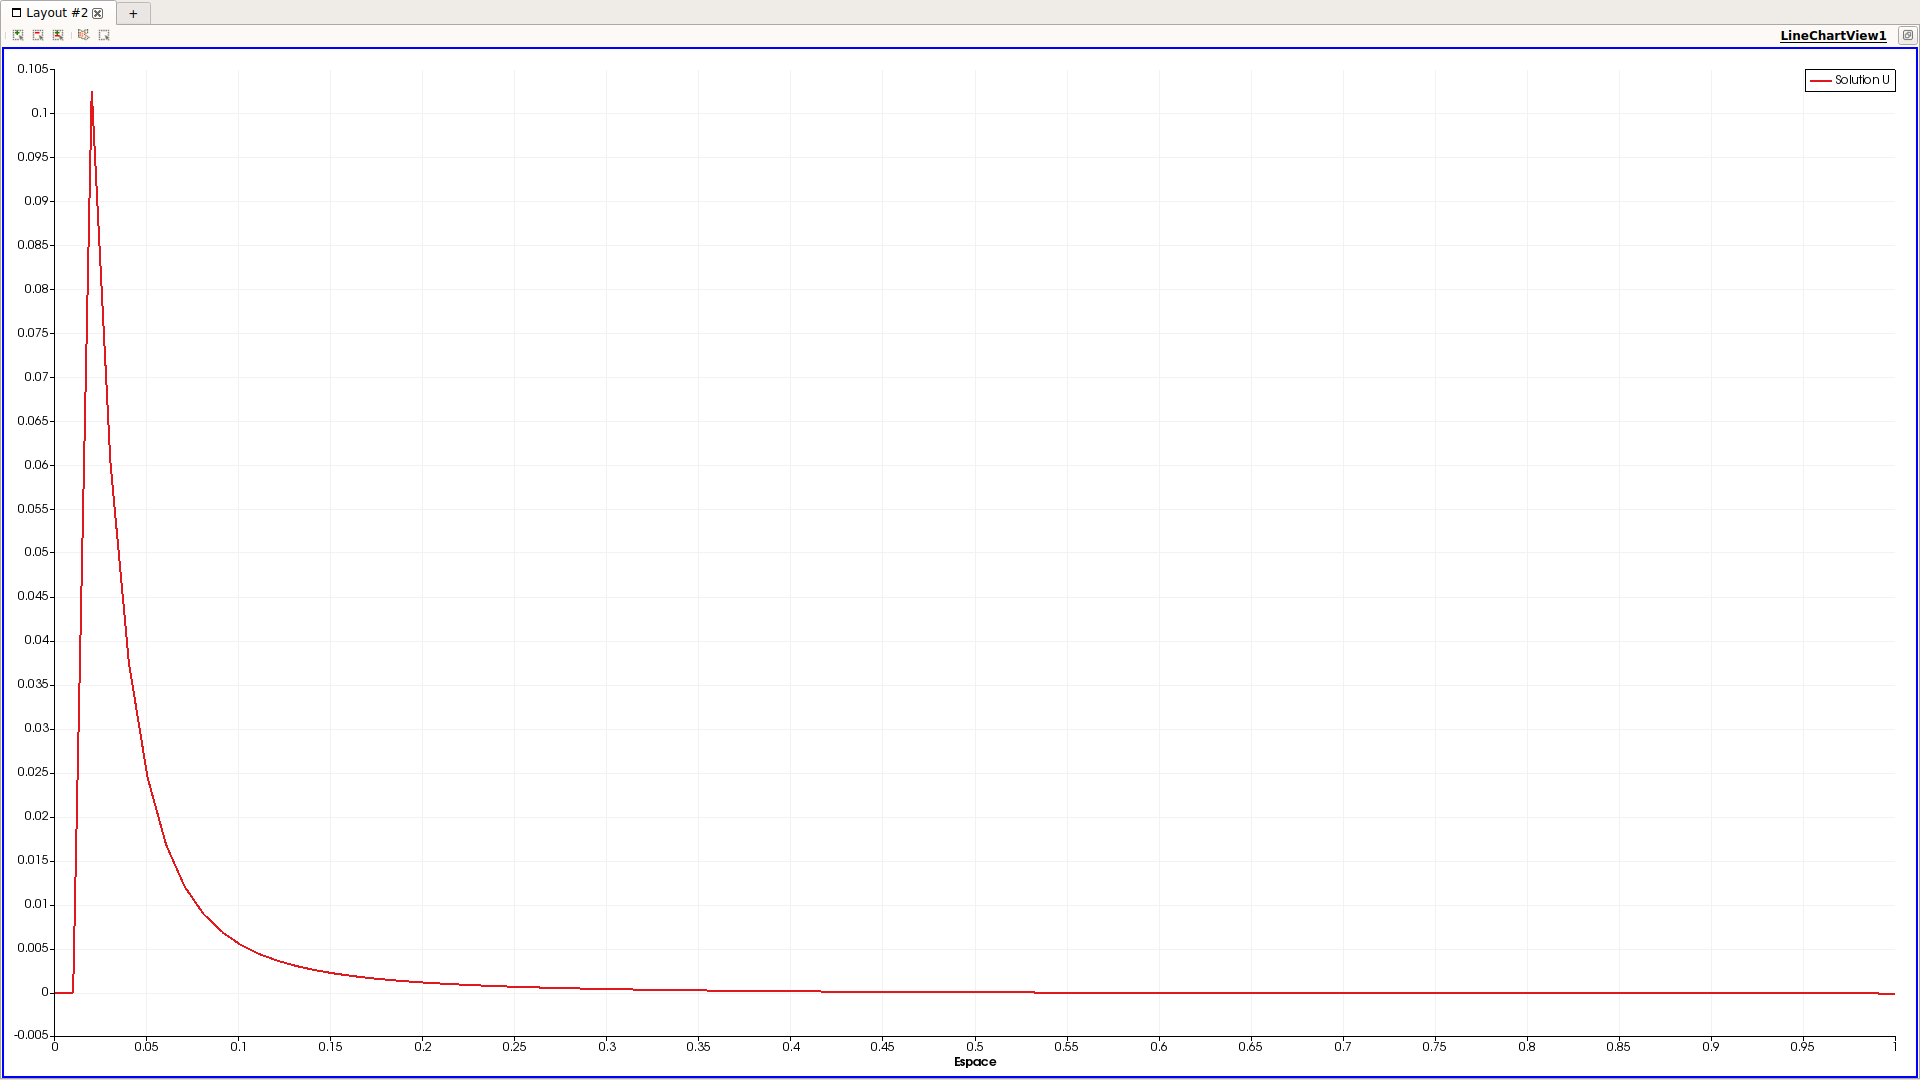
\includegraphics[scale=0.2]{image.png}
\end{document}
